\documentclass[11pt,letterpaper]{article}
\usepackage{amsmath, amssymb, amsbsy}
\usepackage{cite, graphicx}
\usepackage{geometry}
\usepackage{subcaption}

\usepackage[usenames,dvipsnames]{xcolor} 

\usepackage[utf8]{inputenc}

\geometry{letterpaper,nohead,margin=1.4in}
\parindent1em
\parskip0pc
\linespread{1.0}
\pagestyle{plain}

\newcommand{\com}[1]{\hspace{2em}\textrm{#1}} % comments
\newcommand{\sinc}[0]{\textrm{sinc}}
\newcommand{\sign}[0]{\textrm{sign}}
\newcommand{\vv}[1]{\mathbf{#1}} % vector
\newcommand{\p}[0]{\mathbb{P}}
\newcommand{\e}[0]{\mathbb{E}}
\newcommand{\var}[0]{\textrm{Var}}

\title{Learning From Data Problems: Chapter II}
\date{}
\author{J. David Giese}

\begin{document}
\maketitle

\section*{Exercise 2.1}
The breaking point for (1) is $N = 2$ because $(1, -1) \not\in \mathcal{H}(\vv{x}_1, \vv{x}_2)$.
\\\\
The breaking point for (2) is $N = 3$ because $(1, -1, 1) \not\in \mathcal{H}(\vv{x}_1, \vv{x}_2, \vv{x}_3)$.
\\\\
There is no breaking point for (3) because every dichotomy can be generated by $\mathcal{H}$.

\section*{Exercise 2.2}

a) For (1), we have $m_\mathcal{H}(N) \le \binom{N}{1} + \binom{N}{0} = N + 1$, which is true.
\\\\
For (2), we have $m_\mathcal{H}(N) \le \binom{N}{2} + \binom{N}{1} + \binom{N}{0} = N^2/2 + N/2 + 1$, which is true.
\\\\
There is no bound for (3) as there is no break point.
\\\\
b) No, because if $m_\mathcal{H}(N) < 2^N$ then there must be a break point, however if there is a break point it will be polynomial bounded.

\section*{Exercise 2.3}
The Vapnik-Chervonenkis dimension is 1, 2, and $\infty$ respectively.

\section*{Exercise 2.4}
a) First we select $\mathcal{D}$ such that the samples, when placed in the rows of a matrix form:
\begin{align*}
    G &= 
    \begin{bmatrix}
        1 & \mathbf{0} \\
        \mathbf{1} & \mathbf{I}_d
    \end{bmatrix}
    \intertext{where $\mathbf{I}_d$ is the $d \times d$ identity matrix.  We can see by inspection that $G$ is invertible, however for fun we can use a matrix identity to prove it:}
    \textrm{det}\begin{pmatrix}
        A & B \\
        C & D
    \end{pmatrix}
    &= 
    \textrm{det}(A)
    \textrm{det}(D - CA^{-1}B) \quad \Longrightarrow \\
    \textrm{det}(G) &= \textrm{det}(1)\textrm{det}(I_d - \vv{1}\times\vv{0}) = 1.
\end{align*}
We can thus solve $\vv{b} = G\vv{w}$ given a weight vector $\vv{w}$, and can generate each dichotomy by selecting the sign of each dimension of $\vv{b}$.
\\\\
b) Select our first $d + 1$ points as in (a).  Clearly the $d + 2$ point will be a linear combination of the first points (because we have already spanned the space).  This means we we no longer have enough free parameters to vary $\vv{b}$ and generate each dichotomy.

\section*{Exercise 2.5}
\begin{align*}
    \delta &= 4 m_\mathcal{H}(2 N) \exp (-N\epsilon^2/8) \\
    &\le 4 ((2N)^{d_\textrm{vc}} + 1) \exp (-N\epsilon^2/8) \\
    &= 4((2\cdot 100) + 1) \exp(-100 (0.1)^2 / 8) \\
    &\approx 709.
\end{align*}
Clearly, although $\delta$ is a probability, the bound we have set for it can be much greater than 1, and thus useless.

\section*{Exercise 2.6}
a) The Hoeffding Inequality on the test data gives the bound $\epsilon = \sqrt{\frac{1}{2\cdot200}\ln \frac{2}{0.05}} = 0.096$.  We can also use the Hoeffding Inequality for the trained bound, because the hypothesis set is finite; in other words, we don't need to resort to the VC bound.  We have $\epsilon = \sqrt{\frac{1}{2\cdot400}\ln\frac{2\cdot1000}{0.05}} = 0.115$.  The bound provided by the test data is clearly better.
\\\\
b) This is a subtle question.  Note we are not changing $\mathcal{H}$ so it is not a trade off between model complexity and in-sample error.  Looking out the simple generalization bound with $M = 1$
\begin{align*}
    E_\textrm{out}(g) &\le E_\textrm{in}(g) + \sqrt{\frac{1}{2N}\ln\frac{2}{\delta}}
\end{align*}
we see that for a given single hypothesis $g$, using a larger test sample size further tightens the bound.  One may then jump to the conclusion that your in-sample error will take a penalty, however this is not necessarily the case.  In the extreme case (e.g. when you have a single training sample) your $E_\textrm{in}$ is likely to be perfect, because your hypothesis has enough free dimensions to fit the data. Clearly this is still not a good thing, although our mathematical analysis presented in this chapter insufficient to account for it.
\\\\
This appears to exemplify how over-fitting is a separate issue that must also be accounted for.  Clearly, by taking too many samples from our training-set, we will be unable to select the proper $g$, even if the in-sample error is low.

\section*{Exercise 2.7}
a) The squared distance between 0 and 1 is 1, hence the pointwise mean-squared error is equivalent "binary error-measure" used in Chapter 1.
\\\\
b) In this case, the squared distance between -1 and 1 is 4, hence you will need to normalize by 4 to make the pointwise measures equivalent.

\section*{Exercise 2.8}
a) The expectation operator is linear, hence if $\mathcal{H}$ is closed under linear combinations, then $\bar{g} \in \mathcal{H}$.
\\\\
b) If we let $\mathcal{X} = \mathcal{Y} = \mathbb{R}$ and $\mathcal{H} = {1, 0}$ then, unless one of the hypothesis occurs with probability 0, $\bar{g}$ will not be in $\mathcal{H}$.
\\\\
c) No.

\section*{Problem 2.1}
a) $N \ge 840$
\\\\
b) $N \ge 1761$
\\\\
c) $N \ge 2682$

\section*{Problem 2.2}
First note that $\mathcal{X} = \mathbb{R}^2$ is implied by the learning model.  We see an example in Figure \ref{fig:p2_2_1} of four points that are shattered by the hypothesis set of rectangles.  Intuitively this makes sense, as we have four degrees of freedom.
\begin{figure}[]
    \centering
    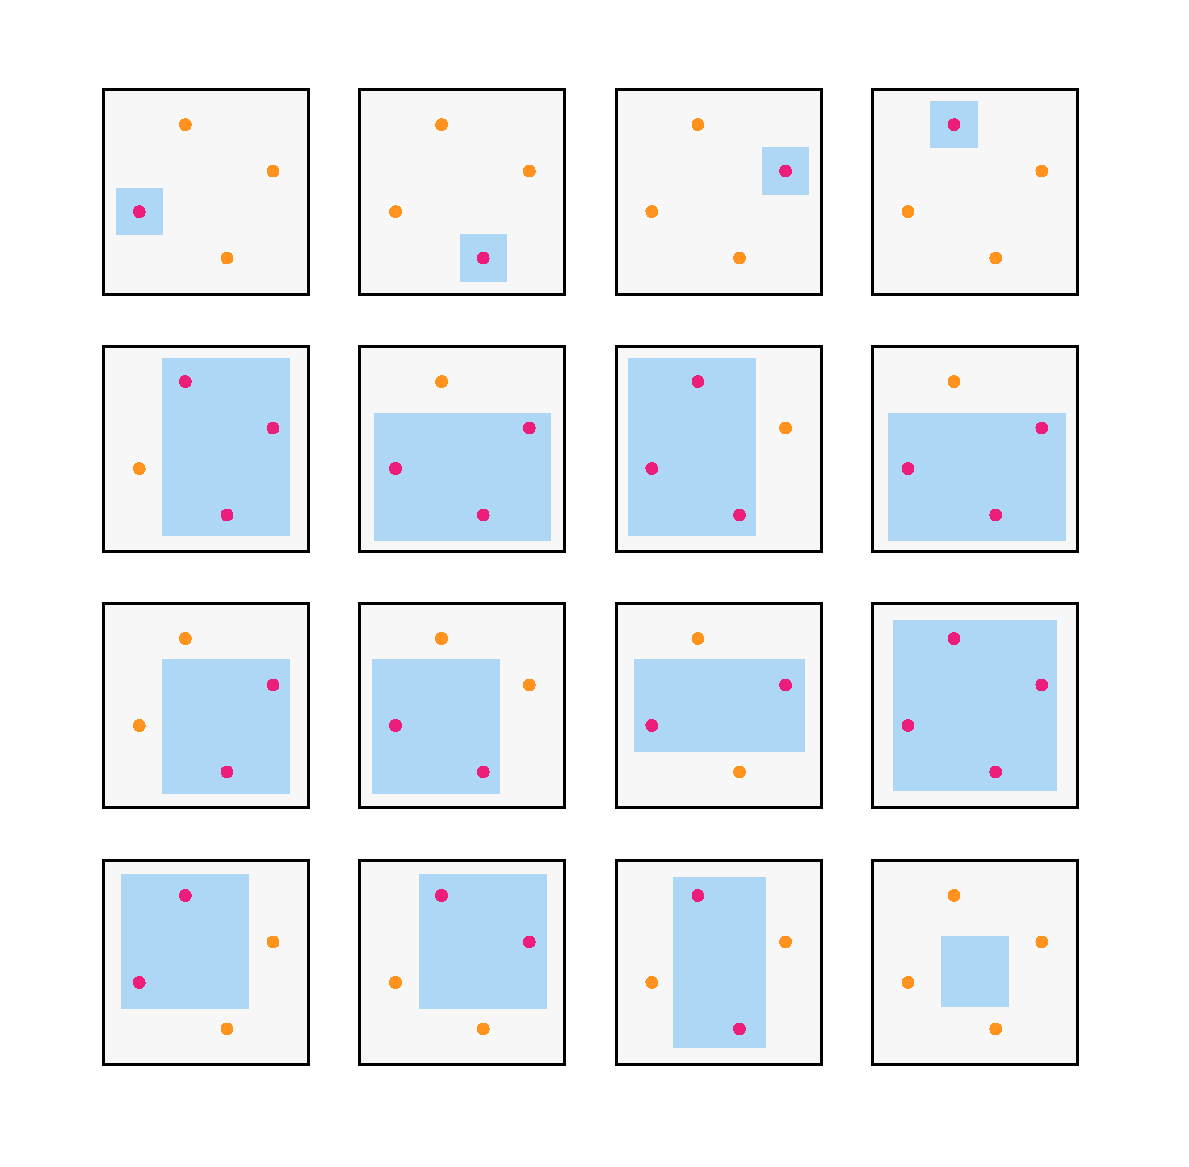
\includegraphics[width=0.8\linewidth]{problem_2_2_a.pdf}
    \caption{Demonstrating that the hypothesis set of positive rectangles is capable of shattering four points.}
    \label{fig:p2_2_1}
\end{figure}
Proving that a rectangle can not shatter five points is a bit tricker.  We do not attempt a formal proof here, but provide a high level overview of how one may approach proving such a thing.  Figure \ref{fig:p2_2_2} illustrates the approach.

\begin{enumerate}
    \item Any set of points such that two are vertically or horizontally aligned can not produce all dichotomies.
    \item Given any set of five ``non-aligned'' points, one can draw a rectangle such there is one point touching at least three sides of the rectangle, and the one or two points are outside this rectangle.
    \item If four points are touching (A), it is impossible to produce the dichotomy wherein the outer point is enveloped, but the point on the adjacent side is not (B).  One may suspect that they can move this point out of the way (C), however by doing this they will always break the first assumption (if the point is on the corner) or they will break the second assumption and they will need to redefine their original rectangle (D), and thus we are no better off then not having moved the point in the first place.
    \item If three points are touching (E) then we run into the same problem with both outside points.
    \item We thus see that is impossible to shatter a set of five points.
\end{enumerate}

We can thus bound our growth function: $m_\mathcal{H}(N) \le N^4 + 1$.

\begin{figure}[]
    \centering
    \centering
    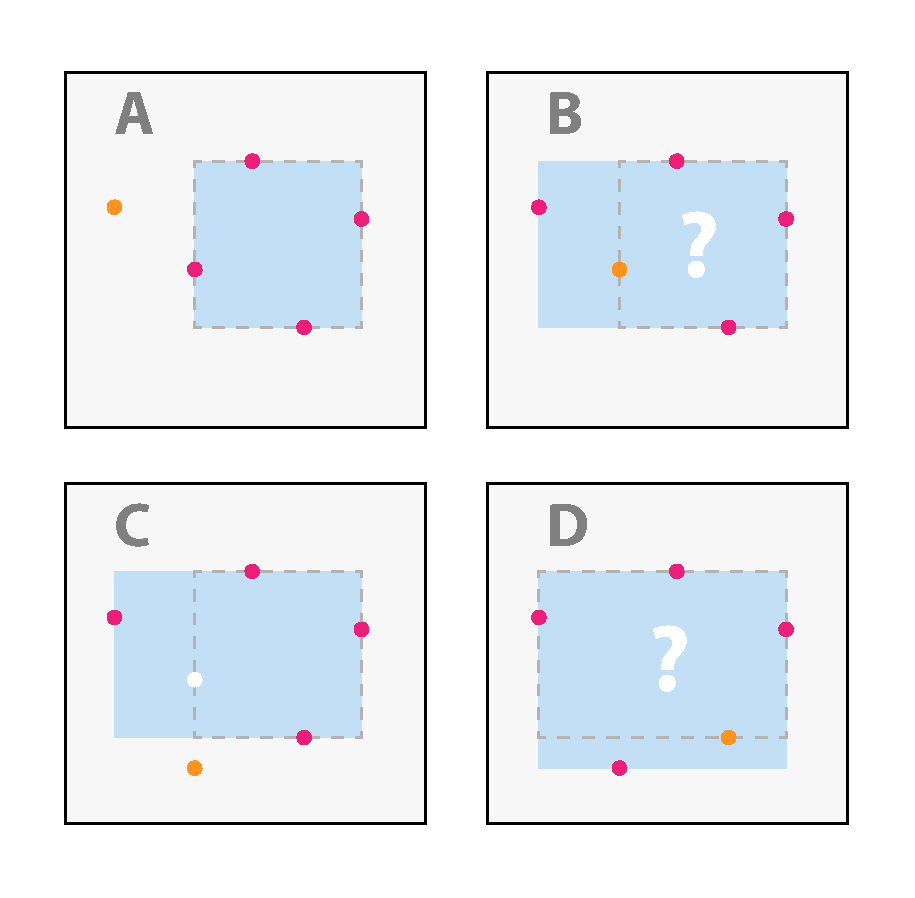
\includegraphics[width=0.8\textwidth]{problem_2_2_b.pdf}
    \caption{Outline of a proof demonstrating that the hypothesis set of positive rectangles can not shatter five points.}
    \label{fig:p2_2_2}
\end{figure}

\end{document}

